\subsection{Panorama Discovery} \label{sec:PanDiscExpSec}

Panorama discovery is defined as finding frames in a video that constitutes a panorama.
The solution may be subjective.  An example is shown in Figure (\ref{fig:archResults}).
An argument can be made that there should be only one panorama.  However, the quality of the 
panorama may suffer due to the motion model error.  The parameters can be tuned, specifically
$\delta$ and $\beta$, to get different results.

The implemented panorama discovery algorithm is robust enough to account for the 
video zoom.  An example is shown in Figure (\ref{fig:vancouverResults}).

\end{multicols}

\begin{figure} [t]
	\centering
	\subfigure[Panorama 1.]{
		\centering
		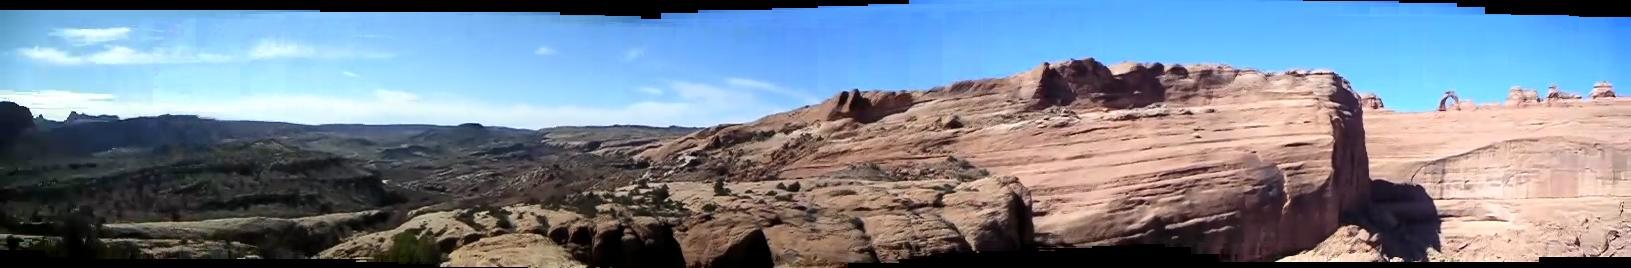
\includegraphics[width=170mm,height=30mm]{archPan1.jpg}  
		\label{fig:archPan1}
	}	
	\subfigure[Panorama 2.]{
		\centering
		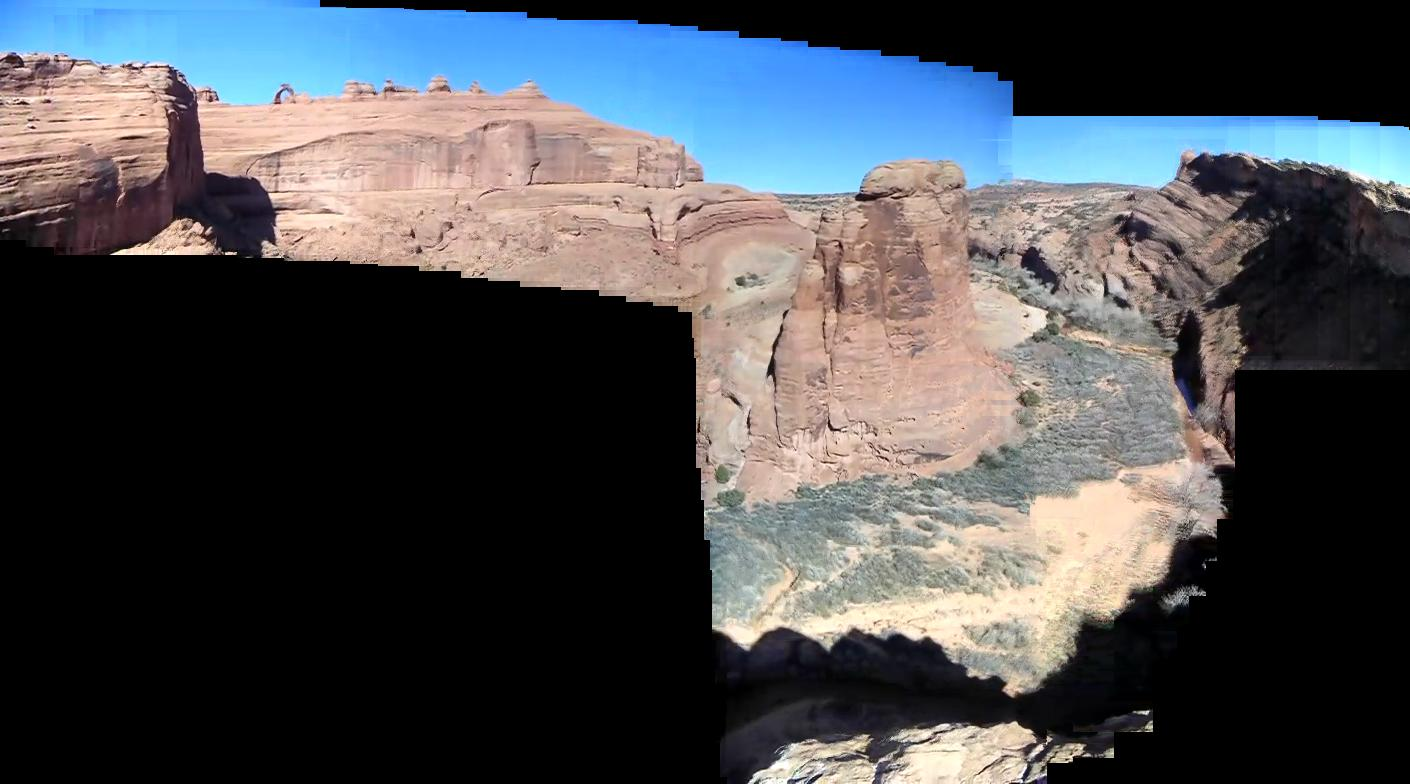
\includegraphics[width=170mm,height=80mm]{archPan2.jpg}  
		\label{fig:archPan2}	
	}
	\caption{Discovered Panoramas from a Web Video \cite{Arches}.} \label{fig:archResults}	
\end{figure}

\begin{figure} [H]
	\centering
	\subfigure[Panorama 1.]{
		\centering
		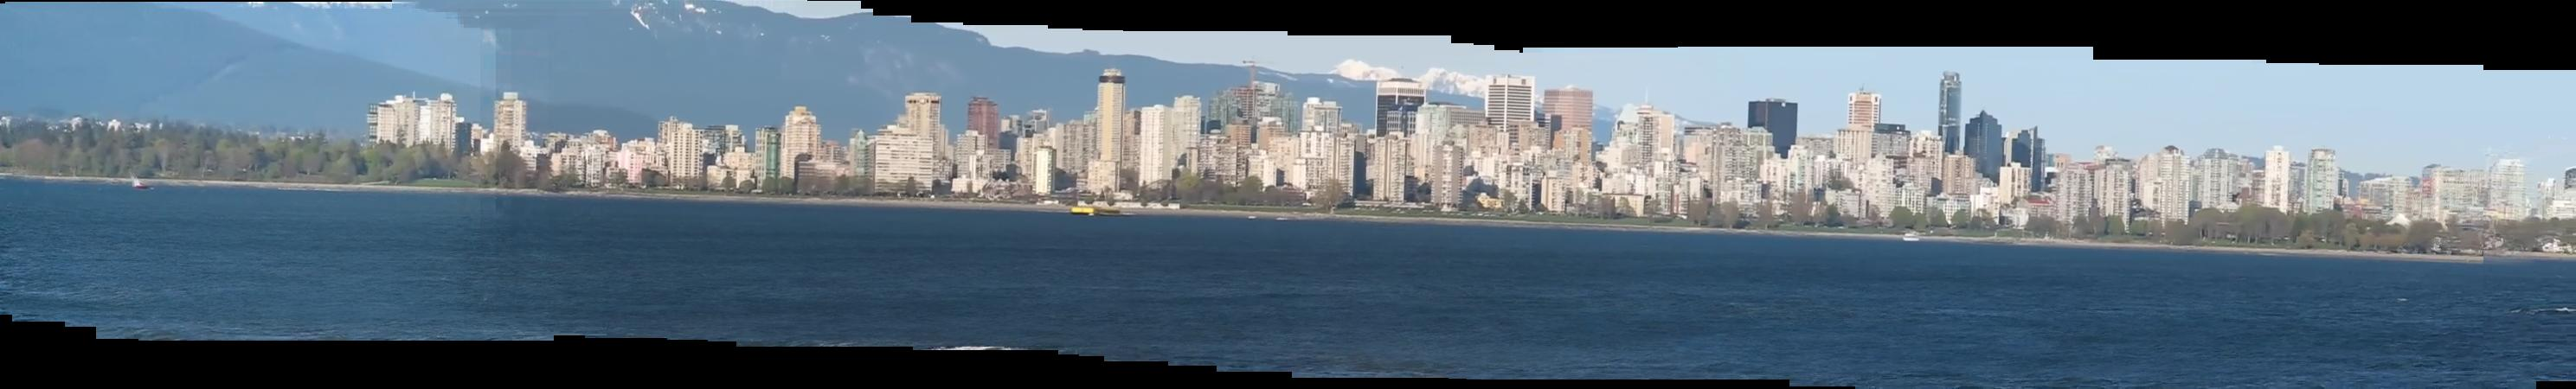
\includegraphics[width=170mm,height=30mm]{vancouverPan1.jpg}  
		\label{fig:vancouverPan1}
	}	
	\subfigure[Panorama 2.]{
		\centering
		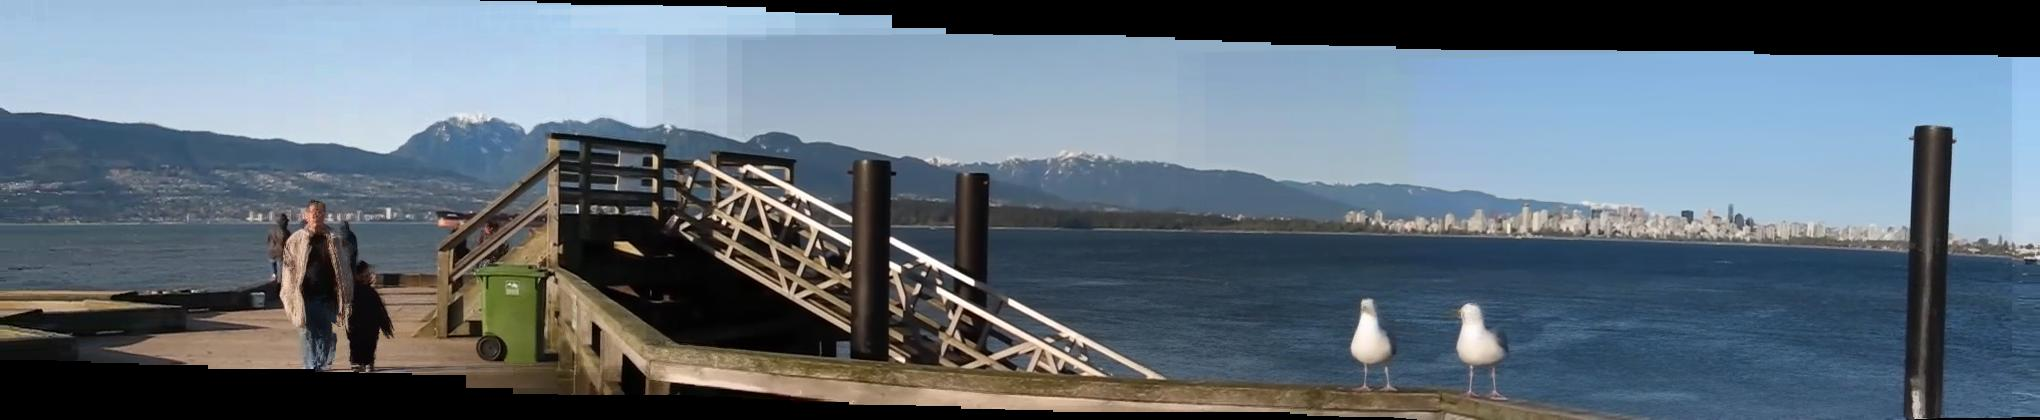
\includegraphics[width=170mm,height=30mm]{vancouverPan2.jpg}  
		\label{fig:vancouverPan2}	
	}
	\caption{Discovered Panoramas from a Web Video \cite{Vancouver}.} \label{fig:vancouverResults}	
\end{figure}

\begin{multicols}{2}